\section{条件未来与局部转移}
\label{sec:ctsp-markov}

第~\ref{chap:discrete-time-stochastic-processes}章用一步转移核$P$描述Markov链：给定当前状态，下一步的条件分布是$P(x,\cdot)$，$n$步转移是核的$n$次复合。连续时间没有“一步”，本节先把转移推广为任意时长$t$的核族，再用短时间内的变化率——生成元——概括这一族核。有限或可数状态的跳跃链让这些对象都变成可以直接计算的矩阵。最后讨论在随机时刻停止后，过程能否像在固定时刻那样重新开始。

\subsection{转移半群与生成元}
\label{sec:ctsp-semigroup}

\paragraph{任意时长的转移核}
设$X$在可测状态空间$(E,\mathcal E)$中取值，并适应于滤过$(\mathcal F_t)$。若存在一族概率核$P_t$，$t\geq0$，使
\begin{equation}
  \mathbb P(X_{s+t}\in A\mid\mathcal F_s)=P_t(X_s,A)\qquad\text{几乎必然},\quad s,t\geq0,\ A\in\mathcal E,
  \label{eq:ctsp-markov-property}
\end{equation}
就称$X$是相对于该滤过的时间齐次Markov过程，$P_t$称为转移核。条件只依赖经过的时长$t$，不依赖出发时刻$s$；若依赖$s$，就要用双参数核$P_{s,s+t}$，下面的讨论平行推广。

对两段时长连续转移，可以用条件期望的塔式性质把它们拼接起来。对$A\in\mathcal E$，
\[
  \begin{aligned}
    P_{s+t}(X_0,A)&=\mathbb E\bigl[\mathbb P(X_{s+t}\in A\mid\mathcal F_s)\bigm|\mathcal F_0\bigr]\\
    &=\mathbb E[P_t(X_s,A)\mid\mathcal F_0]=\int P_s(X_0,\mathrm dy)\,P_t(y,A).
  \end{aligned}
\]
于是转移核满足连续时间的Chapman--Kolmogorov关系
\begin{equation}
  P_{s+t}=P_sP_t,\qquad P_0(x,\cdot)=\delta_x ,
  \label{eq:ctsp-chapman-kolmogorov}
\end{equation}
其中右端是核的复合。时长相加对应核的复合，这是离散关系$P^{m+n}=P^mP^n$的连续版本。

两个基本例子都可以直接核对。Poisson过程从状态$i$出发，经过时长$t$到达$j\geq i$的概率为$P_t(i,\{j\})=e^{-\lambda t}(\lambda t)^{j-i}/(j-i)!$；Brownian运动从$x$出发，经过时长$t$的位置服从$\mathcal N(x,t)$，转移密度为
\begin{equation}
  p_t(x,y)=\frac1{\sqrt{2\pi t}}\exp\Bigl\{-\frac{(y-x)^2}{2t}\Bigr\}.
  \label{eq:ctsp-heat-kernel}
\end{equation}
对Brownian运动，式~\eqref{eq:ctsp-chapman-kolmogorov}就是两个独立高斯增量之和的分布：$\mathcal N(0,s)$与$\mathcal N(0,t)$卷积为$\mathcal N(0,s+t)$。

时间齐次说的是转移规则不随出发时刻改变，不是说$X_t$的分布不变。Brownian运动时间齐次，但$W_t\sim\mathcal N(0,t)$的分布不断铺开；只有当初始分布恰为不变分布时，边缘分布才保持不变，这是第~\ref{sec:ctsp-invariant}节的问题。

\paragraph{半群作用于测试函数与分布}
与离散时间一样，转移核可以从两侧作用。作用在有界可测函数$f$上，
\[
  (P_tf)(x)=\int f(y)\,P_t(x,\mathrm dy)=\mathbb E_x f(X_t),
\]
它回答“从$x$出发，经过时长$t$后读数$f$的平均是多少”。作用在初始分布$\mu$上，$\mu P_t(A)=\int\mu(\mathrm dx)P_t(x,A)$是时刻$t$的状态分布。两种写法由$\langle\mu P_t,f\rangle=\langle\mu,P_tf\rangle$联系，其中$\langle\mu,f\rangle=\int f\,\mathrm d\mu$。式~\eqref{eq:ctsp-chapman-kolmogorov}说明$P_{s+t}f=P_s(P_tf)$，所以$(P_t)_{t\geq0}$构成一个线性算子的\term{转移半群}（transition semigroup）。它还是正的压缩：$f\geq0$时$P_tf\geq0$，并且$\|P_tf\|_\infty\leq\|f\|_\infty$。

\paragraph{生成元：短时间变化率}
离散链由一步核$P$完全确定。连续时间的半群由什么确定？有限状态时答案最清楚。若状态空间有限，$P_t$是随机矩阵，并且$t\mapsto P_t$可微，则由$P_{t+h}=P_tP_h$，
\[
  \frac{P_{t+h}-P_t}h=P_t\,\frac{P_h-\bm I}h\longrightarrow P_t\bm Q,\qquad
  \bm Q=\lim_{h\downarrow0}\frac{P_h-\bm I}h .
\]
于是$P_t$满足矩阵微分方程$\dot P_t=P_t\bm Q$，$P_0=\bm I$，解为矩阵指数$P_t=e^{t\bm Q}$。一个矩阵$\bm Q$就决定了整族转移，它记录的是短时间内各转移概率的变化率。

一般状态空间仍采用同一思路，但必须交代极限在什么意义下取，对哪些函数存在。

\begin{definition}[半群的生成元]
  \label{def:ctsp-generator}
  设$\mathcal B$是一个由有界函数组成、在范数$\|\cdot\|_\infty$下完备的空间，半群$P_t$把$\mathcal B$映入自身，并且强连续：对每个$f\in\mathcal B$，$\|P_hf-f\|_\infty\to0$（$h\downarrow0$）。若极限
  \[
    \mathcal Lf=\lim_{h\downarrow0}\frac{P_hf-f}h
  \]
  在$\|\cdot\|_\infty$中存在，就称$f$属于定义域$\mathcal D(\mathcal L)$，称$\mathcal L$为半群的\term{生成元}（generator）。
\end{definition}

生成元的定义域通常不是全体函数。对Brownian运动取$\mathcal B$为在无穷远处趋于零的连续函数，若$f$二阶连续可微且$f,f',f''$都在无穷远处趋于零，则对固定$x$作Taylor展开，
\[
  \mathbb Ef(x+W_h)-f(x)=f'(x)\,\mathbb EW_h+\tfrac12f''(x)\,\mathbb EW_h^2+o(h)=\tfrac h2f''(x)+o(h),
\]
余项关于$x$一致的估计由$f''$的一致连续性给出。所以$\mathcal Lf=\frac12f''$。不可微的函数不在定义域中；把$\frac12\frac{\mathrm d^2}{\mathrm dx^2}$形式地作用到任意函数上，并不能保证差商极限存在。Poisson过程的生成元则是差分算子$\mathcal Lf(i)=\lambda[f(i+1)-f(i)]$：短时间内只有“跳一格”这一种变化，其概率约为$\lambda h$。

生成元与半群之间的基本关系是两个微分方程。

\begin{theorem}[Kolmogorov方程]
  \label{thm:ctsp-kolmogorov-equations}
  在定义~\ref{def:ctsp-generator}的条件下，若$f\in\mathcal D(\mathcal L)$，则对每个$t\geq0$，$P_tf\in\mathcal D(\mathcal L)$，并且
  \[
    \frac{\mathrm d}{\mathrm dt}P_tf=\mathcal LP_tf=P_t\mathcal Lf ,
  \]
  导数在$\|\cdot\|_\infty$意义下理解。
\end{theorem}

\begin{proof}
由半群性质，$h^{-1}(P_{t+h}f-P_tf)=P_t\bigl(h^{-1}(P_hf-f)\bigr)$。$P_t$是压缩，所以右端在$\|\cdot\|_\infty$中收敛到$P_t\mathcal Lf$。同一个量也等于$h^{-1}(P_h-I)(P_tf)$，它收敛说明$P_tf\in\mathcal D(\mathcal L)$且极限为$\mathcal LP_tf$。以上是右导数；左导数由$h^{-1}(P_tf-P_{t-h}f)=P_{t-h}\bigl(h^{-1}(P_hf-f)\bigr)$，并利用$\|P_{t-h}\mathcal Lf-P_t\mathcal Lf\|_\infty\to0$（强连续性）同样得到。
\end{proof}

$\frac{\mathrm d}{\mathrm dt}P_tf=\mathcal LP_tf$称为\term{后向方程}（backward equation），它关于出发点$x$的变量求导；对Brownian运动，它就是热方程$\partial_tu=\frac12\partial_{xx}u$，$u(t,x)=\mathbb E_xf(X_t)$，与第~\ref{chap:partial-differential-equations}章研究的扩散方程是同一个对象。作用在分布一侧得到\term{前向方程}（forward equation），它描述密度怎样流动，将在第~\ref{sec:ctsp-backward-forward}节与随机微分方程一起讨论。

\subsection{连续时间Markov链}
\label{sec:ctsp-ctmc}

\paragraph{停留时间与跳转概率}
状态空间可数时，可以用一个具体的机制生成连续时间Markov过程。处在状态$i$时，过程先停留一段随机时间，然后跳到另一个状态。停留时间必须是指数分布：只有指数分布具有无记忆性，才能保证“已经停留了多久”不影响未来，使当前状态概括全部相关历史。

具体地，给每个状态$i$一个离开率$q_i\geq0$和跳转分布$(p_{i,j})_{j\neq i}$。过程在$i$停留$\operatorname{Exp}(q_i)$时间，然后以概率$p_{i,j}$跳到$j$，再在$j$重复同样的步骤；各次停留和选择相互独立。记
\begin{equation}
  q_{i,j}=q_ip_{i,j}\ (j\neq i),\qquad q_{i,i}=-q_i=-\sum_{j\neq i}q_{i,j},
  \label{eq:ctsp-q-matrix}
\end{equation}
矩阵$\bm Q=(q_{i,j})$称为\term{生成矩阵}（generator matrix）。非对角元非负，每行之和为零。

同一机制还有一个等价的画面：在状态$i$，为每个可能的目标$j$各开一只独立的闹钟，响铃时间服从$\operatorname{Exp}(q_{i,j})$，最先响的那只决定跳向哪里。独立指数变量的最小值服从速率为$\sum_jq_{i,j}=q_i$的指数分布，并且第$j$只最先响的概率为$q_{i,j}/q_i=p_{i,j}$，与最小值本身独立。所以$q_{i,j}$可以读作“从$i$流向$j$的速率”：短时间$h$内从$i$跳到$j$的概率约为$q_{i,j}h$。图~\ref{fig:ctsp-ctmc-path}给出一个三状态例子的速率图和一条路径。

\begin{figure}[htbp]
  \centering
  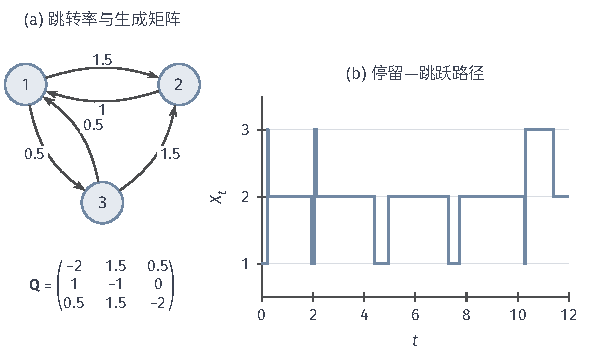
\includegraphics[width=105mm]{figures/03-optimization-evolution-and-signals/02-processes-and-trajectory-evolution/tikz/ctsp-ctmc-path/figure.pdf}
  \caption{三状态连续时间Markov链。(a)箭头上的数是跳转率$q_{i,j}$，生成矩阵的对角元是负的离开率，每行之和为零；(b)从状态$1$出发的一条路径（固定随机种子）：在每个状态停留一段指数时间后跳走，状态$2$只能跳回$1$，离开率最小，因而平均停留最久。}
  \label{fig:ctsp-ctmc-path}
\end{figure}

只看跳跃发生的先后顺序，记$Y_0,Y_1,Y_2,\ldots$为依次访问的状态，就得到一条离散时间Markov链，转移矩阵为$(p_{i,j})$，称为\term{嵌入跳链}（embedded jump chain）。连续时间链等于这条离散链再配上依赖当前状态的指数停留时间。第~\ref{sec:ctsp-occupation}节将看到，两者长期访问各状态的比例可以不同。

\paragraph{矩阵指数与前后向方程}
有限状态时，由构造可以直接验证短时间转移概率：从$i$出发，$h$内不跳的概率为$e^{-q_ih}=1-q_ih+O(h^2)$，恰好跳一次到$j$的概率为$q_{i,j}h+O(h^2)$，跳两次以上的概率为$O(h^2)$。于是$P_h=\bm I+h\bm Q+O(h^2)$，转移概率满足
\begin{equation}
  P_t=e^{t\bm Q},\qquad
  \dot P_t=\bm QP_t\ \text{（后向方程）},\qquad
  \dot P_t=P_t\bm Q\ \text{（前向方程）}.
  \label{eq:ctsp-ctmc-kolmogorov}
\end{equation}
后向方程来自把$[0,t+h]$拆成先走$h$再走$t$，前向方程来自先走$t$再走$h$。若行向量$\bm\mu_t$表示时刻$t$的分布，则$\bm\mu_t=\bm\mu_0P_t$满足$\dot{\bm\mu}_t=\bm\mu_t\bm Q$，逐个分量写出就是
\[
  \frac{\mathrm d}{\mathrm dt}\mu_t(j)=\sum_{i\neq j}\mu_t(i)q_{i,j}-\mu_t(j)q_j ,
\]
即流入$j$的概率流减去流出$j$的概率流。分布不随时间改变当且仅当$\bm\pi\bm Q=\bm0$。

\begin{example}[两态链的转移概率]
  \label{ex:ctsp-two-state}
  取状态$\{1,2\}$，离开$1$的率为$a$，离开$2$的率为$b$，$\bm Q=\begin{pmatrix}-a&a\\b&-b\end{pmatrix}$。$\bm Q$的特征值为$0$和$-(a+b)$，计算矩阵指数得
  \[
    P_t=\frac1{a+b}\begin{pmatrix}b+ae^{-(a+b)t}&a-ae^{-(a+b)t}\\b-be^{-(a+b)t}&a+be^{-(a+b)t}\end{pmatrix}.
  \]
  可以直接核对$P_0=\bm I$与$\dot P_t=\bm QP_t$。$t\to\infty$时两行都趋于$\bm\pi=(b,a)/(a+b)$，且$\bm\pi\bm Q=\bm0$。初值的影响按$e^{-(a+b)t}$消退，速率由$\bm Q$的非零特征值决定。取$a=1,b=2$，得$\bm\pi=(2/3,1/3)$：离开率较小的状态$1$占据更多时间。
\end{example}

\paragraph{可数状态与爆炸}
状态可数无限时，局部速率$\bm Q$还不一定决定一个在所有时刻都有定义的过程。记第$n$次跳跃时刻为$J_n=S_0+\cdots+S_{n-1}$，其中$S_k$是第$k$段停留。若$J_\infty=\lim_nJ_n<\infty$，过程在有限时间内跳了无穷多次，之后的状态没有被构造规定，这称为\term{爆炸}（explosion）。

\begin{example}[纯生过程的爆炸]
  \label{ex:ctsp-explosion}
  在$\{0,1,2,\ldots\}$上只允许$i\to i+1$，离开率$q_i=2^i$。停留时间$S_i\sim\operatorname{Exp}(2^i)$相互独立，$\mathbb EJ_\infty=\sum_i2^{-i}=2<\infty$，所以$J_\infty<\infty$几乎必然：过程在平均两个时间单位内跑遍所有状态。若$q_i=\lambda$为常数，$\mathbb EJ_\infty=\infty$，并且由强大数律$J_n/n\to1/\lambda$，不会爆炸；这正是Poisson计数。
\end{example}

一般地，$J_\infty=\infty$几乎必然当且仅当$\sum_n1/q_{Y_n}=\infty$几乎必然，其中$Y$是嵌入跳链\scite{math-kallenberg2021probability}。由此得到两个常用的充分条件：离开率有界；或嵌入跳链常返，使某个$q_i>0$的状态被访问无穷多次。只给出局部速率时，应当先检查不爆炸，或明确采用在$J_\infty$处停止的“最小过程”；不能把“速率已经给定”等同于“完整过程已经构造好”。

\paragraph{出生死亡链}
很多计数模型只允许状态每次增减一。设状态$k$处的出生率为$\lambda_k$（$k\to k+1$），死亡率为$\mu_k$（$k\to k-1$，$\mu_0=0$），这就是\term{出生死亡链}（birth--death chain）。$\mu_k\equiv0$、$\lambda_k\equiv\lambda$时它退化为Poisson计数；$\lambda_k\equiv\lambda$、$\mu_k\equiv\mu$（$k\geq1$）时，它描述单服务台排队的队长：顾客以速率$\lambda$到来，服务以速率$\mu$完成。

出生死亡链的平衡分布可以由相邻状态之间的概率流平衡求出。在$k$与$k+1$之间，单位时间内从$k$上行的平均次数为$\pi_k\lambda_k$，从$k+1$下行的平均次数为$\pi_{k+1}\mu_{k+1}$。令二者相等，
\begin{equation}
  \pi_k\lambda_k=\pi_{k+1}\mu_{k+1},\qquad
  \pi_k=\pi_0\prod_{j=0}^{k-1}\frac{\lambda_j}{\mu_{j+1}} .
  \label{eq:ctsp-birth-death-balance}
\end{equation}
这是连续时间的细致平衡。对每个$j$，$(\bm\pi\bm Q)_j=\pi_{j-1}\lambda_{j-1}-\pi_j(\lambda_j+\mu_j)+\pi_{j+1}\mu_{j+1}$，把细致平衡的两个等式代入，各项两两抵消，所以它蕴含$\bm\pi\bm Q=\bm0$。排队例中$\pi_k=(1-\rho)\rho^k$，$\rho=\lambda/\mu$，只有$\rho<1$时求和归一化才可能；$\rho\geq1$时队长没有平衡分布，平均意义下会无限增长或零常返地游荡。图~\ref{fig:ctsp-birth-death}画出了$\rho=0.6$的情形。这个模型的速率不超过$\lambda+\mu$，所以不会爆炸。

\begin{figure}[htbp]
  \centering
  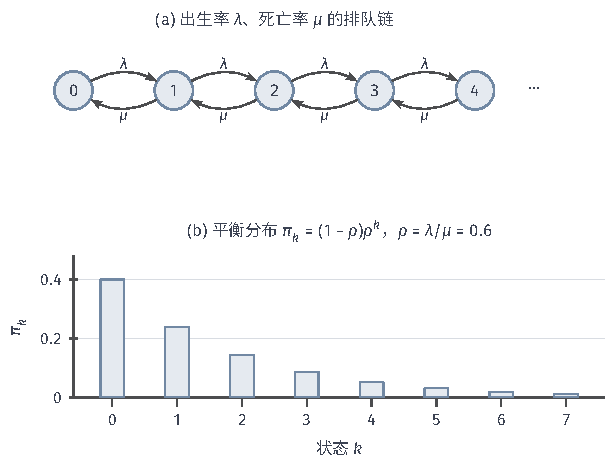
\includegraphics[width=105mm]{figures/03-optimization-evolution-and-signals/02-processes-and-trajectory-evolution/tikz/ctsp-birth-death/figure.pdf}
  \caption{单服务台排队的出生死亡链。(a)上行箭头为到达率$\lambda$，下行箭头为服务率$\mu$，状态$0$不能再下行；(b)$\rho=\lambda/\mu=0.6$时由细致平衡得到的几何平衡分布$\pi_k=(1-\rho)\rho^k$，只画出$k\leq7$。}
  \label{fig:ctsp-birth-death}
\end{figure}

\subsection{停止后的Markov过程}
\label{sec:ctsp-strong-markov}

\paragraph{离散证明为何不能照搬}
第~\ref{chap:discrete-time-stochastic-processes}章证明了离散链的\term{强Markov性质}（strong Markov property）：在停时$\tau$处，给定$\mathcal F_\tau$，过程从$X_\tau$重新开始，后续规律与从该状态出发的链相同。证明把事件按$\{\tau=n\}$分解，在每一块上使用普通Markov性质，再对$n$求和。连续停时可以取不可数多个值，每个取值的概率都可能为零，这种分解失效。本小节用式~\eqref{eq:ctsp-dyadic-stopping}的离散逼近绕过这一困难，并说明为此需要哪些路径和半群条件。

\paragraph{Brownian运动的强Markov性质}
先看最重要的情形。

\begin{theorem}[Brownian运动的强Markov性质]
  \label{thm:ctsp-brownian-strong-markov}
  设$W$是相对于满足通常条件的滤过的标准Brownian运动，$\tau$是停时且$\mathbb P(\tau<\infty)=1$。则$B_t=W_{\tau+t}-W_\tau$，$t\geq0$，是标准Brownian运动，并且独立于$\mathcal F_\tau$。
\end{theorem}

\begin{proof}
固定时刻$0\leq t_1<\cdots<t_m$、有界连续函数$g:\mathbb R^m\to\mathbb R$和$A\in\mathcal F_\tau$，只需证明
\begin{equation}
  \mathbb E[g(B_{t_1},\ldots,B_{t_m})\mathbb I_A]=\mathbb E\,g(W_{t_1},\ldots,W_{t_m})\cdot\mathbb P(A).
  \label{eq:ctsp-strong-markov-target}
\end{equation}
取$\tau_n$如式~\eqref{eq:ctsp-dyadic-stopping}，记$B^{(n)}_t=W_{\tau_n+t}-W_{\tau_n}$。因为$\tau\leq\tau_n$，$A\in\mathcal F_\tau\subseteq\mathcal F_{\tau_n}$，从而$A\cap\{\tau_n=k2^{-n}\}\in\mathcal F_{k2^{-n}}$。在这一块上，$B^{(n)}$就是固定时刻$k2^{-n}$之后的增量过程，独立于$\mathcal F_{k2^{-n}}$并且是标准Brownian运动。对可数个$k$求和，
\[
  \begin{aligned}
    \mathbb E[g(B^{(n)}_{t_1},\ldots,B^{(n)}_{t_m})\mathbb I_A]
    &=\sum_k\mathbb E\,g(W_{t_1},\ldots,W_{t_m})\,\mathbb P(A\cap\{\tau_n=k2^{-n}\})\\
    &=\mathbb E\,g(W_{t_1},\ldots,W_{t_m})\,\mathbb P(A).
  \end{aligned}
\]
令$n\to\infty$。路径连续且$\tau_n\downarrow\tau$，所以$B^{(n)}_{t_i}\to B_{t_i}$逐点成立；$g$有界连续，由控制收敛定理左端趋于式~\eqref{eq:ctsp-strong-markov-target}的左端。有限维分布与独立性因此成立；$B$的路径连续直接继承自$W$。
\end{proof}

证明中两个条件各有分工。停时性质保证$A\cap\{\tau_n=k2^{-n}\}$在时刻$k2^{-n}$已知，从而可以使用固定时刻的独立增量；路径连续保证离散逼近的极限就是停时处的值。对一般Markov过程，第二步需要把$P_tf(X_{\tau_n})$的极限传到$P_tf(X_\tau)$，这要求路径右连续，并且$x\mapsto P_tf(x)$对连续的$f$仍连续。满足后一条件（并在无穷远处保持趋零）的半群称为Feller半群，具有右连续路径的Feller过程都满足强Markov性质\scite{math-kallenberg2021probability}。连续时间Markov链在跳跃时刻重新开始，则直接由停留—跳跃的构造得到。

\paragraph{普通Markov性质不够}
没有路径与半群的正则条件，强Markov性质可能失效。设$\xi\sim\operatorname{Exp}(1)$，令$X_t=(t-\xi)^+$：过程在$0$处停留一段指数时间，然后以单位速度向右移动。由指数分布的无记忆性，它对每个固定时刻都满足Markov性质，转移规则是“在$0$处等待一段$\operatorname{Exp}(1)$时间后离开，在正半轴上匀速右移”。但在右连续滤过下，$\tau=\inf\{t:X_t>0\}=\xi$是停时，$X_\tau=0$，而过程在$\tau$之后立刻离开$0$，不会再等待一段指数时间。从$X_\tau$重新开始的规律与转移核给出的规律不同。问题出在半群的连续性上：对连续的$f$，$x>0$时$P_tf(x)=f(x+t)$，在$x\downarrow0$时趋于$f(t)$，而$P_tf(0)=\mathbb Ef((t-\xi)^+)$一般不等于$f(t)$。$P_tf$在零点不连续，Feller条件不成立，离散逼近的极限步骤因此无法完成。

\paragraph{反射原理}
强Markov性质的价值在于它把“首次到达之后”的路径变成一个新的、可以计算的Brownian运动。设$a>0$，$\tau_a=\inf\{t:W_t=a\}$。由路径连续，$W_{\tau_a}=a$。在$\tau_a$之后，路径向上与向下是对称的：由定理~\ref{thm:ctsp-brownian-strong-markov}，$B_s=W_{\tau_a+s}-a$是独立于$\mathcal F_{\tau_a}$的Brownian运动，与$-B$同分布。于是对$t>0$，
\[
  \mathbb P(W_t\geq a)=\mathbb P(\tau_a\leq t,\ B_{t-\tau_a}\geq0)=\tfrac12\,\mathbb P(\tau_a\leq t),
\]
这里使用了$\tau_a$与$B$独立，以及$B$在任何正时刻取正、负值的概率各为一半（取零的概率为零）。记$M_t=\max_{s\leq t}W_s$，由$\{M_t\geq a\}=\{\tau_a\leq t\}$得到
\begin{equation}
  \mathbb P(M_t\geq a)=2\,\mathbb P(W_t\geq a)=2\bigl[1-\Phi(a/\sqrt t)\bigr],
  \label{eq:ctsp-reflection}
\end{equation}
其中$\Phi$是标准正态分布函数。这一结果称为\term{反射原理}（reflection principle）：把首次到达$a$之后的路径关于水平线$a$翻折，终点在$a$上方与下方的路径一一对应。

式~\eqref{eq:ctsp-reflection}给出两个以后会用到的事实。令$t\to\infty$，$\mathbb P(\tau_a<\infty)=1$：Brownian运动必然到达任意给定高度。对$t$求导得$\tau_a$的密度$a(2\pi t^3)^{-1/2}e^{-a^2/(2t)}$，它按$t^{-3/2}$衰减，所以$\mathbb E\tau_a=\infty$。到达是必然的，平均等待却是无穷的；第~\ref{sec:ctsp-optional-sampling}节将看到，这正是可选抽样在这里失效的原因。
